%SECTION MOVED TO IMPLEMENTATION


%\subsection{Motivation}
%The goal of good design is to find the right balance between a set of parameters, which usually include efficiency, weight and aesthetics. For a long time, this process had been an ardous loop of minute modifications to the product, oscillating between the engineer and the designer. However, with the advent of Topology optimization (see \autoref{sec:TopOpt}) and additive manufacturing, it has been shrunk drastically to an efficient, compact task. In the previous section, we summarized the different ways of representing a design object digitally. On specifying the appropriate loads as boundary conditions on this object, one can choose their favourite topology optimization tool to compute the optimal dimensions and form.


%The main hurdle with most state-of-the-art open source topology optimization tools is their input format, where many of them require input to be specified as a 3-dimensional voxel grid. Presence (or absence) of material in these voxels is defined by a boolean variable, and boundary conditions are imposed on the appropriate locations. An example of voxelized data can be seen in \autoref{fig: voxelOpenCascade}. Since there is a variety of toolboxes available which are able to perform a voxelization of common CAD input files, we did not implement one of our own but rather adapted one of the open source tools. For the implementation we refer to \autoref{sec: CADToVoxels}. %This section describes how we overcame this hurdle of converting CAD representations to voxelized input.
%\begin{figure}
%\centering
%  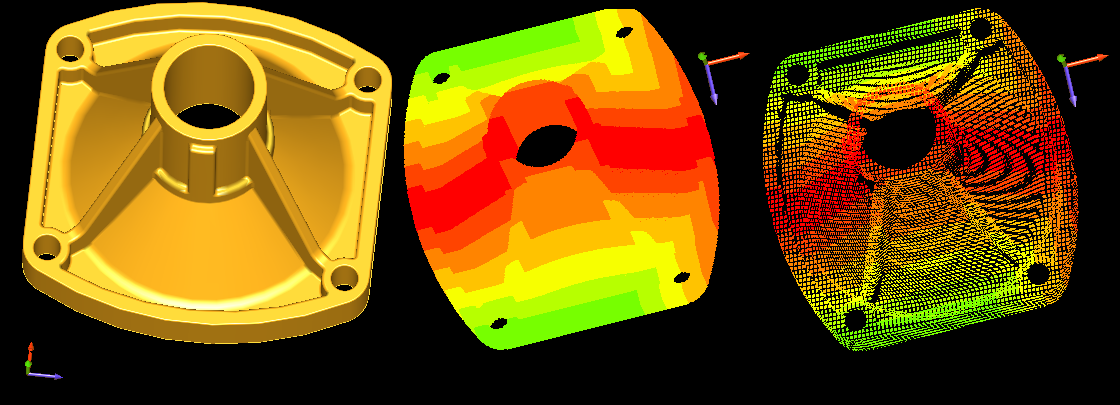
\includegraphics[scale=0.3]{Pictures/CADToVoxel/voxels_wp_image005.png}
%\caption{A shape and its voxel representation. \textem{Leftmost picture}: The original parametrized shape. \textem{Rightmost picture}: The voxel representation. Picture from OpenCascade \cite{OpenCascade}.}
%\label{fig: voxelOpenCascade}
%\end{figure}

 